\clearpage

\section{SOP Modulator}
\label{sec:sop}
\begin{refsection}

\begin{tcolorbox}	
\begin{tabular}{p{2.75cm} p{0.2cm} p{10.5cm}} 	
\textbf{Header File}    &:& sop\_modulator\_*.h \\
\textbf{Source File}    &:& sop\_modulator\_*.cpp \\
\textbf{Version}        &:& 20180514 (Mariana Ramos)
\end{tabular}
\end{tcolorbox}

This block of code simulates a modulation of the State Of Polarization (SOP)in a quantum channel, which intends to insert possible errors occurred during the transmission due the polarization rotation of single photons. These SOP changes can be simulated using deterministic or stochastic methods. The type of simulation is one of the input parameters when the block is initialized.


\subsection*{Functional description}

This block intends to simulate SOP changes using deterministic and stochastic methods. The required function mode must be set when the block is initialized. Furthermore, other input parameters should be also set at initialization. If a deterministic method was set by the user, he also needs to set the $\theta$ and $\phi$ angles in degrees, which corresponds to the two parameters of Jones Space in Poincare Sphere thereby being the rotation and elevation angle, respectively. On the other hand, if a stochastic method is set by the user a model proposed in \cite{Czegledi16} was implemented.

\begin{figure}[H]
    \centering
        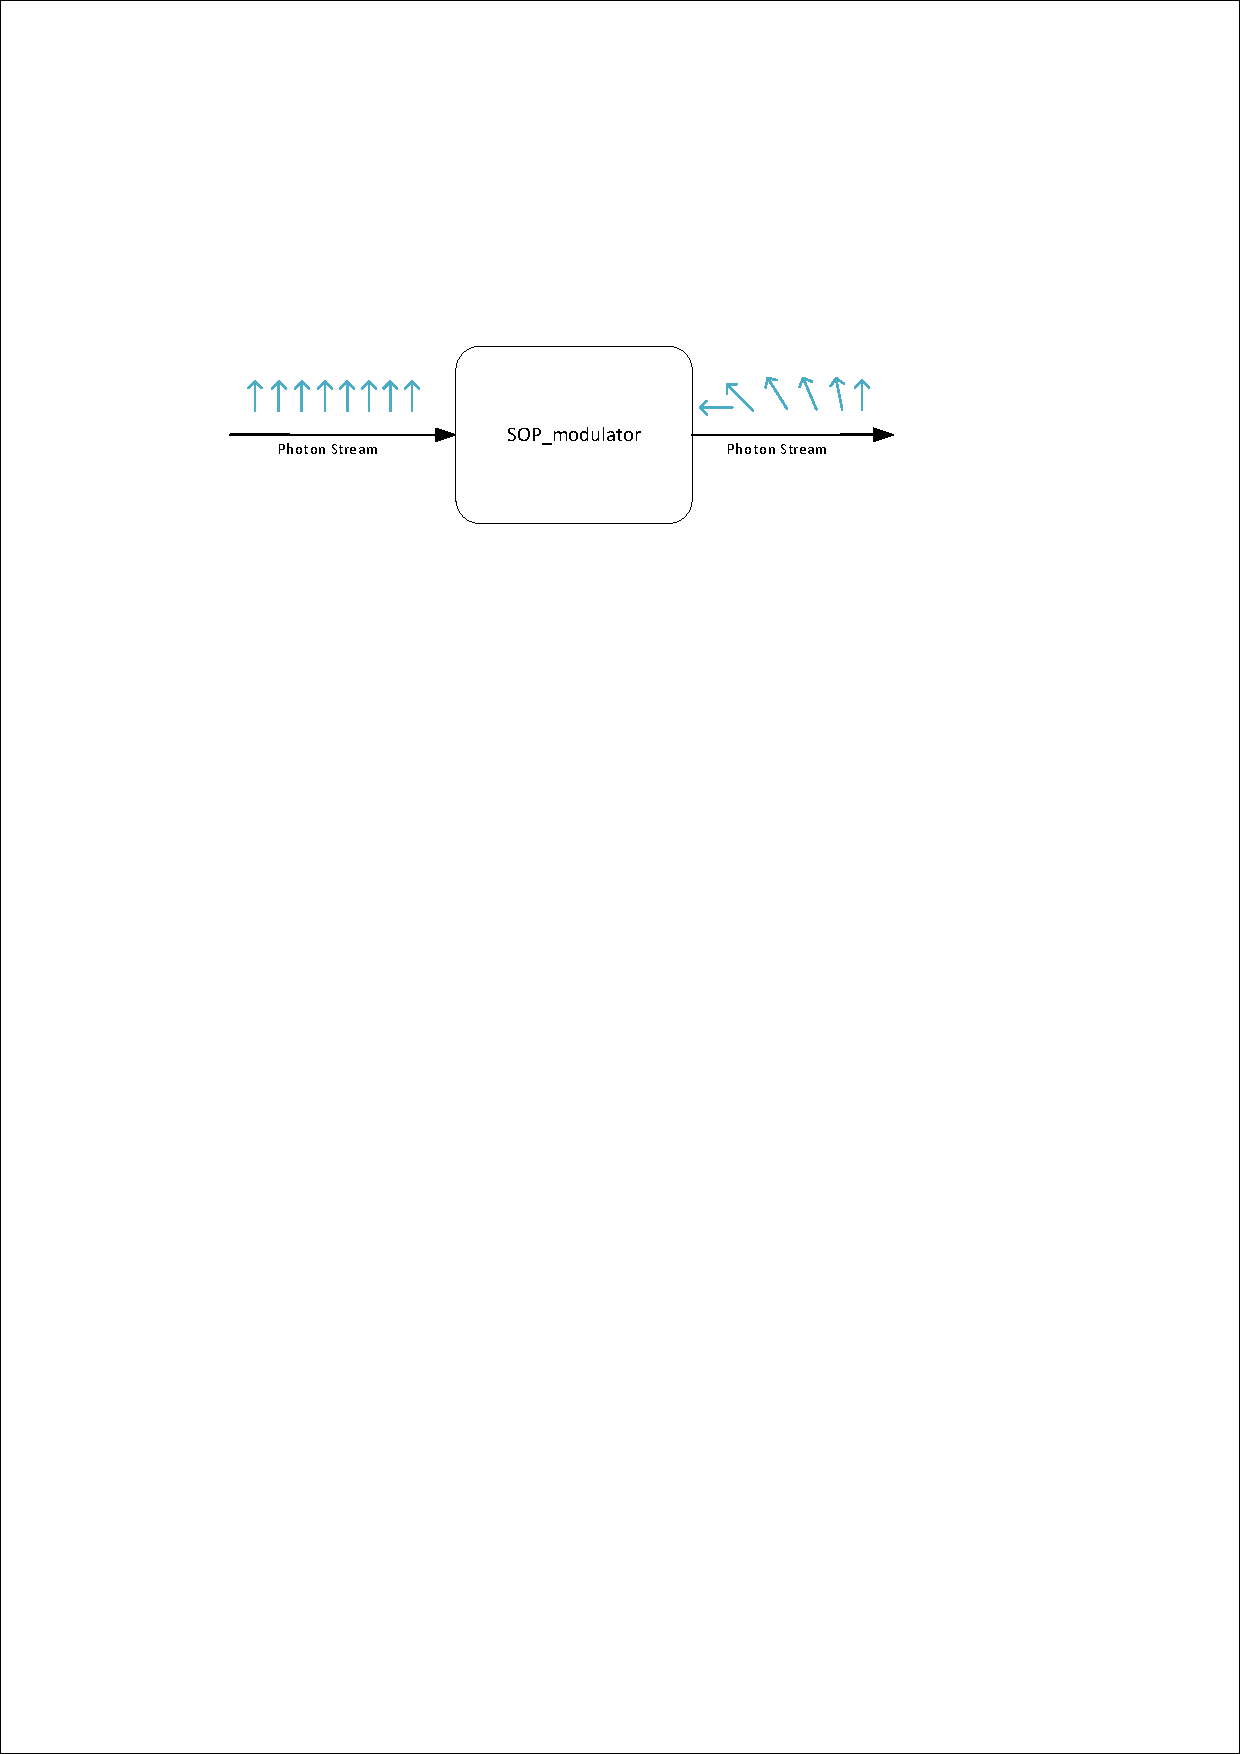
\includegraphics[clip, trim=1cm 20cm 1cm 5.5cm, width=1.00\textwidth]{./lib/sop_modulator/figures/sop.pdf}
    \caption{Diagram block of SOP block input and outputs.}\label{sop}
  \end{figure}

  The block in figure \ref{sop} was implemented based on a continuous matrix calculation. Lets assume that the input photon stream can be represented by the matrix:
  \begin{equation}\label{inputphoton}
  S_{in} =
    \begin{bmatrix}
    A_x \\
    A_y
  \end{bmatrix},
  \end{equation}
  where $A_x$ and $A_y$ are complex numbers. The SOP block will implement the multiplication operation between the input photon $S_{in}$ and the random matrix $\textbf{J}_k$ obtaining the output photon $S_{out}$ with a different polarization:
  \begin{equation}\label{sop_mult}
    S_{out} = S_{in} \textbf{J}_k,
  \end{equation}
  where,
  \begin{equation}\label{eq_jk}
    \textbf{J}_k = J(\pmb{\dot{\alpha}})\textbf{J}_{k-1}.
  \end{equation}
  $J(\pmb{\alpha})$ is a random matrix which can be expressed using the matrix exponential parameterized by $\pmb{\alpha}=(\alpha_1,\alpha_2, \alpha_3)$:
  \begin{eqnarray}
   \nonumber % Remove numbering (before each equation)
    J(\pmb{\alpha})    &=& e^{-i \pmb{{\alpha}} \cdot \pmb{\vec{\sigma}}} \\
                            &=& \textbf{I}_2 \cos(\theta)-i\textbf{a} \cdot \pmb{\vec{\sigma}} \sin(\theta),
  \end{eqnarray}
  where $\pmb{\vec{\sigma}} = (\pmb{\sigma_1}, \pmb{\sigma_2}, \pmb{\sigma_3})$ is the tensor of Pauli Matrices:

  \begin{equation}\label{eqPauli1}
    \pmb{\sigma_1}=
    \begin{bmatrix}
      1 & 0 \\
      0 & -1
    \end{bmatrix};
    \pmb{\sigma_2}=
    \begin{bmatrix}
      0 & 1 \\
      1 & 0
    \end{bmatrix};
    \pmb{\sigma_3}=
    \begin{bmatrix}
      0 & -i \\
      i & 0
    \end{bmatrix}.
  \end{equation}
$\textbf{I}_2$ is the $2 \times 2$ identity matrix. In addition, $\pmb{\alpha} = \theta \pmb{a}$, having the length $\theta = \|\pmb{\alpha}\|$ and the direction on the unit sphere $\pmb{a} = (a_1,a_2,a_3)$, where $\|\cdot\|$ denotes the Euclidian norm. Furthermore, the randomness is achieved by $\pmb{\alpha}$ parameters:

  \begin{equation}\label{eq:alpha}
    \pmb{\dot{\alpha}} \sim \mathcal{N}(0,\sigma_p^2\textbf{I}_3),
  \end{equation}
  where $\sigma_p^2=2\pi \Delta p T$, being $T$ the symbol period and $\Delta p$ the polarization linewidth, which is a parameter dependent on the fiber installation.

  This method allows to analyse the polarization drift over time for a fixed fiber length.


\subsection*{Input parameters}

SOP modulator block must have an input signals to set the clock of the operations. This block has some input parameters that can be manipulated by the user in order to change the basic configuration of the SOP modulator. Each parameter has associated a function that allows for its change. In the following table (table~\ref{table}) the input parameters and corresponding functions are summarized.

\begin{table}[h]
	\begin{center}
		\begin{tabular}{| m{3,5cm} | m{5,8cm} |  m{2,5cm} | m{4cm} | }
			\hline
			\textbf{Input parameters} & \textbf{Function} & \textbf{Accepted values} \\ \hline
			sopType                  & Simulation type that the user intends to simulate. & Deterministic OR Stocastic\\
            theta                       & Rotation Angle in Jones space for deterministic rotation in degrees & double \\
            phi                         & Elevation Angle in Jones space for deterministic rotation in degrees & double \\
            deltaP                      & Polarization Linewidth & double \\
			\hline
		\end{tabular}
		\caption{List of input parameters of the block sop modulator.} \label{table}
	\end{center}
\end{table}


\subsection*{Methods}

SOPModulator(vector <Signal*> \&inputSignals, vector <Signal*> \&outputSignals)(\textbf\{constructor\})
\bigbreak
void initialize(void)
\bigbreak
bool runBlock(void)
\bigbreak
void setSOPType(SOPType sType)
\bigbreak
void setRotationAngle(double angle)
\bigbreak
void setElevationAngle(double angle)
\bigbreak
void setDeltaP(long double deltaP)
\bigbreak
long double getDeltaP()


\pagebreak

\subsection*{Input Signals}

\subparagraph*{Number:} 1

\subparagraph*{Type:} PhotonStreamXY

\subsection*{Output Signals}

\subparagraph*{Number:} 1

\subparagraph*{Type:} PhotonStreamXY

\subsection*{Example}

\subsection*{Sugestions for future improvement}

% bibliographic references for the section ----------------------------
\clearpage
\printbibliography[heading=subbibliography]
\end{refsection}
\addcontentsline{toc}{subsection}{Bibliography}
\cleardoublepage
% ---------------------------------------------------------------------
